\documentclass[12pt]{article}
\usepackage{amsmath}
\usepackage{graphicx}
\title{Report for Auto Control Lab6}
\date{2020/9/29}
\author{Jacky Yeh 4107064003}

\begin{document}
\begin{titlepage}

\maketitle
\end{titlepage}


\section{Introduction}
This is the third Experiment of Auto Control Lab where TAs taught us more of the plot of transfer functions, and the use of combinations of feedback loops.\\

\section{LAB6}
\subsection{Feedback arithmetics and its codes}
Objective:To perform basic operations on different systems and output their results.\\

These are the stated Homework problems\\
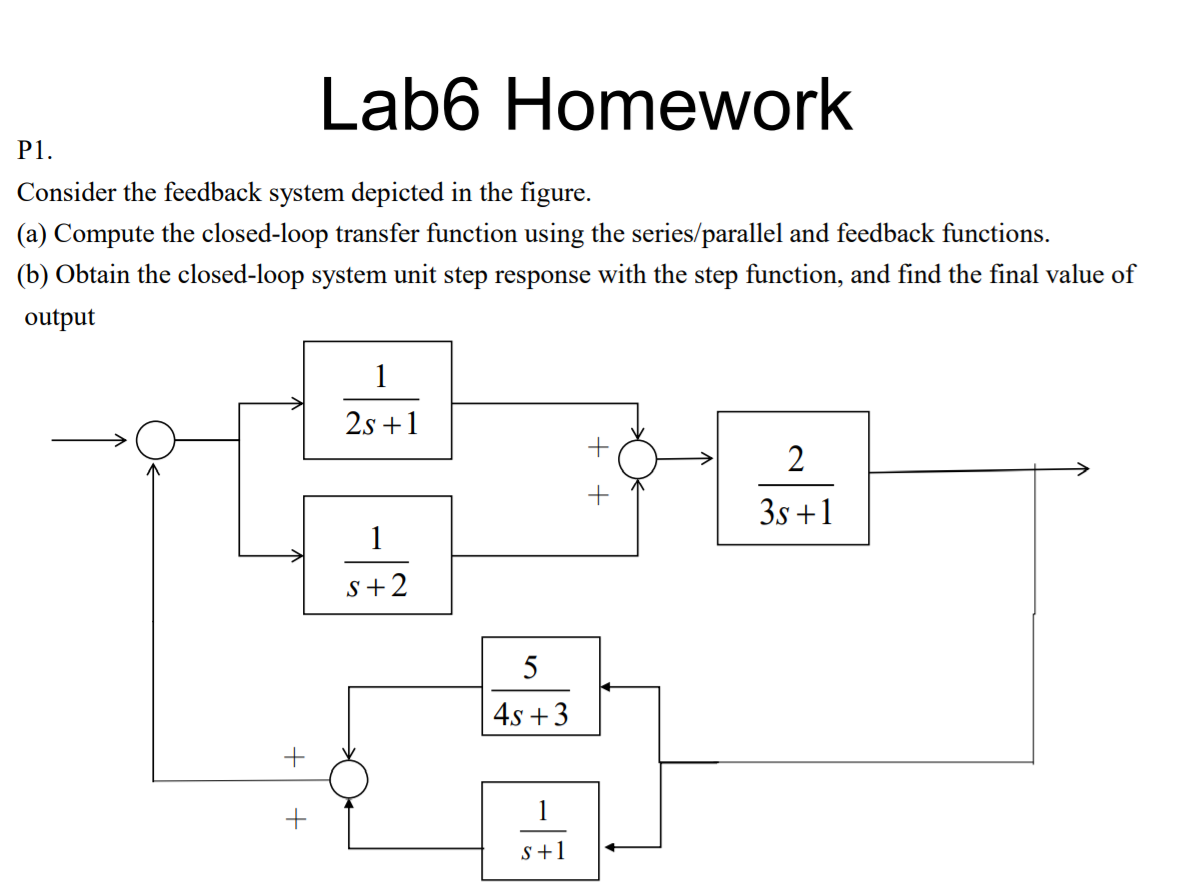
\includegraphics[scale=0.5]{../Lab6/HW_code1.png} \\


\subsection{CODES FOR PROBLEM1}
In order to perform the tasks, Matlab codes are needed. The following is the code needed for generating the transfer function and feedback loops for HW problem 1 \\
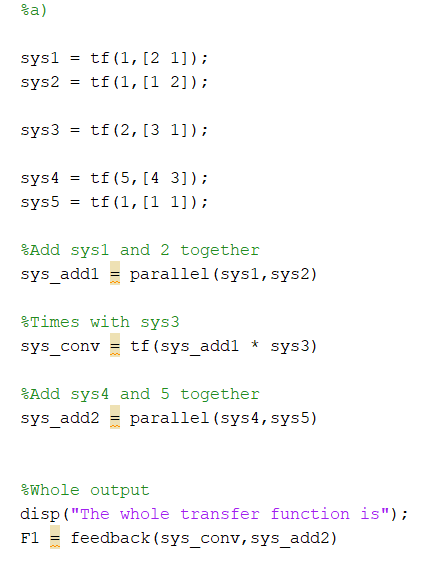
\includegraphics[scale=1]{../Lab6/HW_2_code1.png} \\

\cleardoublepage

\subsection{Results OF the given feedback transfer functions} 
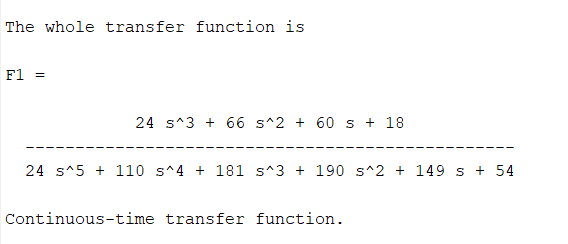
\includegraphics[scale=1]{../Lab6/HW_2_result1.png} \\

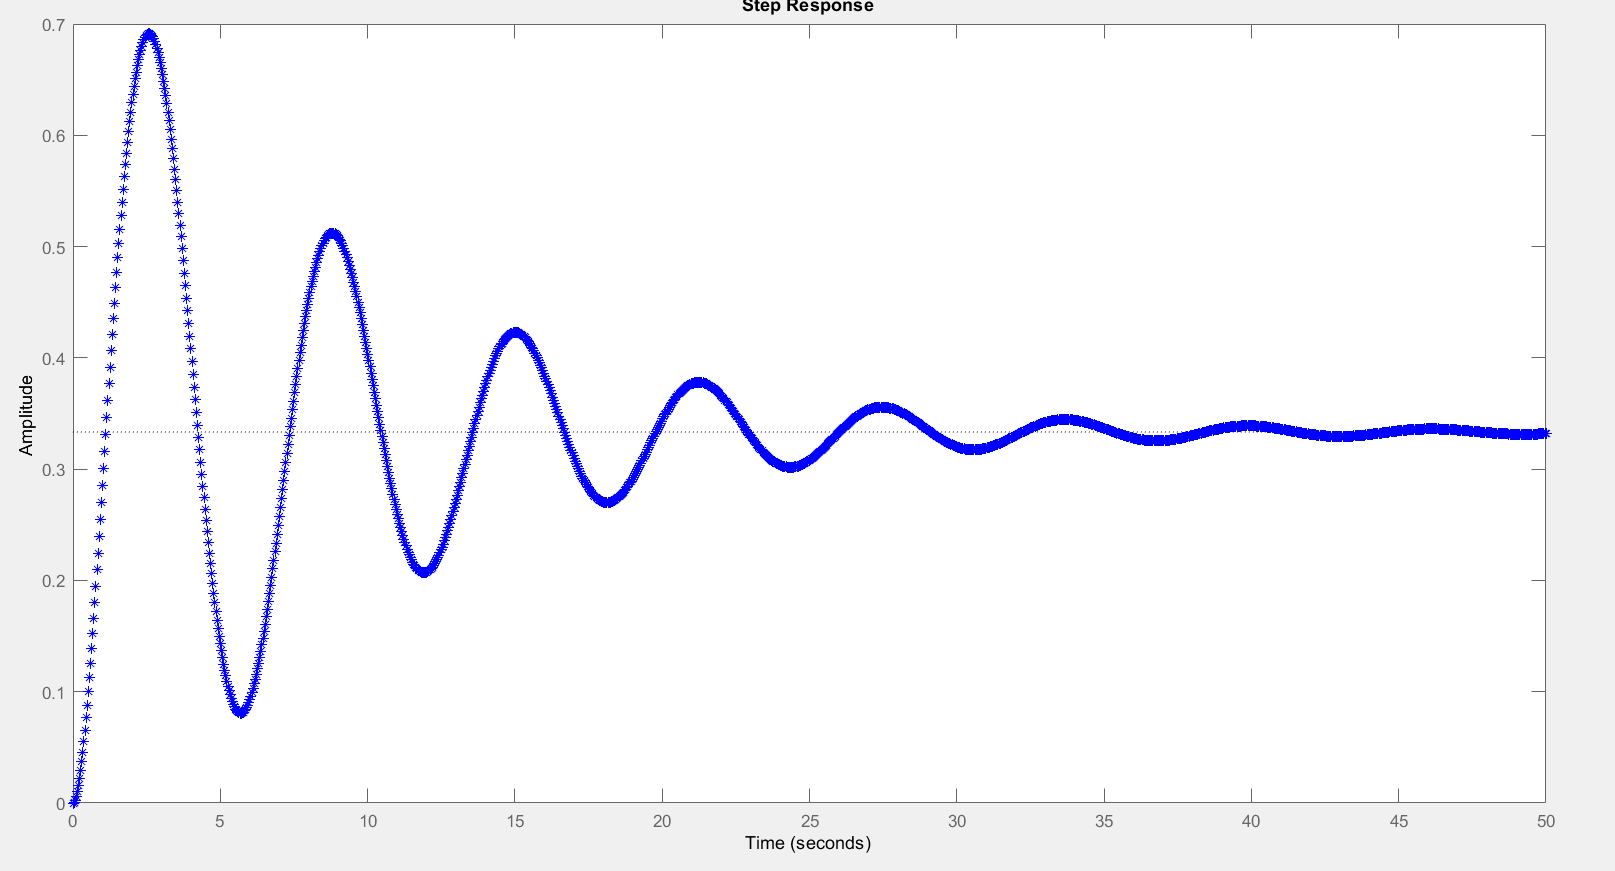
\includegraphics[scale=0.5]{../Lab6/HW_2_result2.png} \\

\cleardoublepage



 
\cleardoublepage
\subsection{PROBLEM2}
Objective:To perform basic operations on different systems and output their results.\\
These are the stated HW problems.

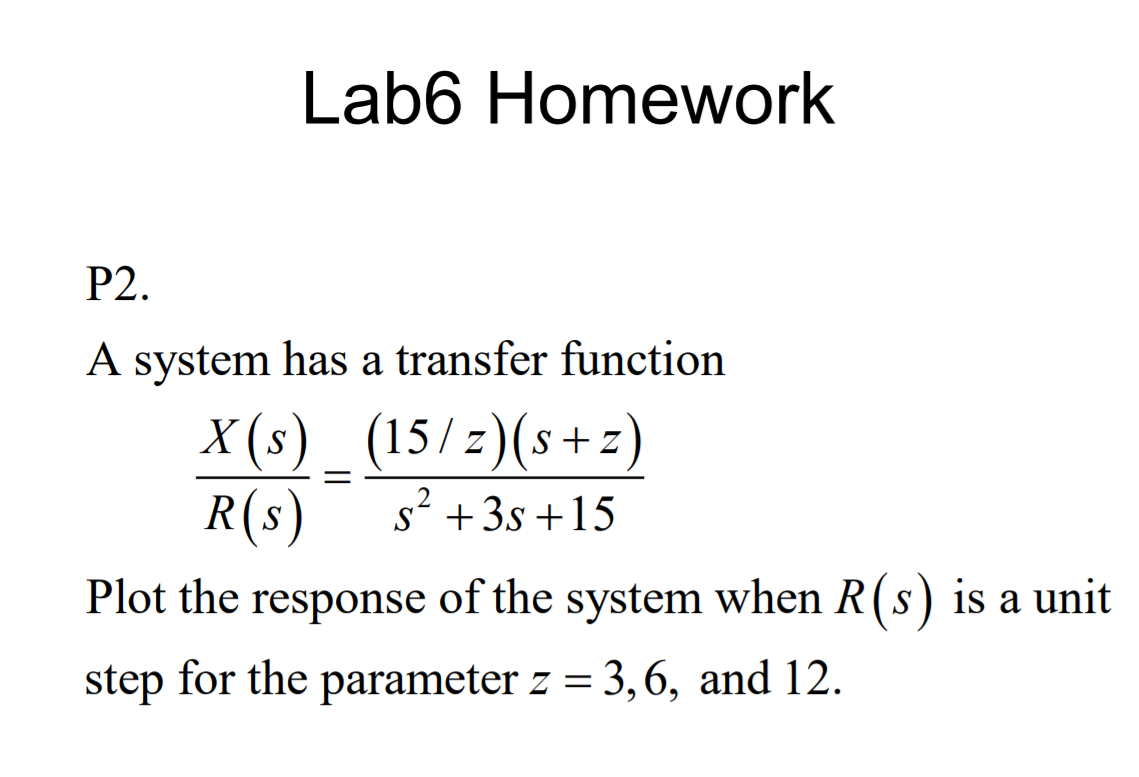
\includegraphics[scale=0.5]{../Lab6/HW_2.png} \\

\cleardoublepage
\subsection{CODES FOR PROBLEM1}
In order to perform the tasks, Matlab codes are needed. The following is the code needed for generating the transfer function of HW problem 2 and output the result as different step response as input\\
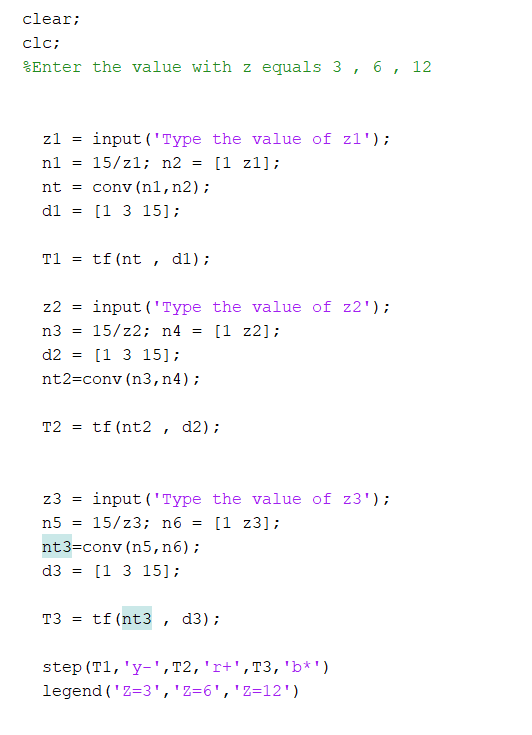
\includegraphics[scale=0.9]{../Lab6/HW_code2.png} \\

\cleardoublepage

\subsection{Plot Results OF the given  transfer functions with different step responses} 
The plots for 3 plots given as z = 3,6,12\\ 
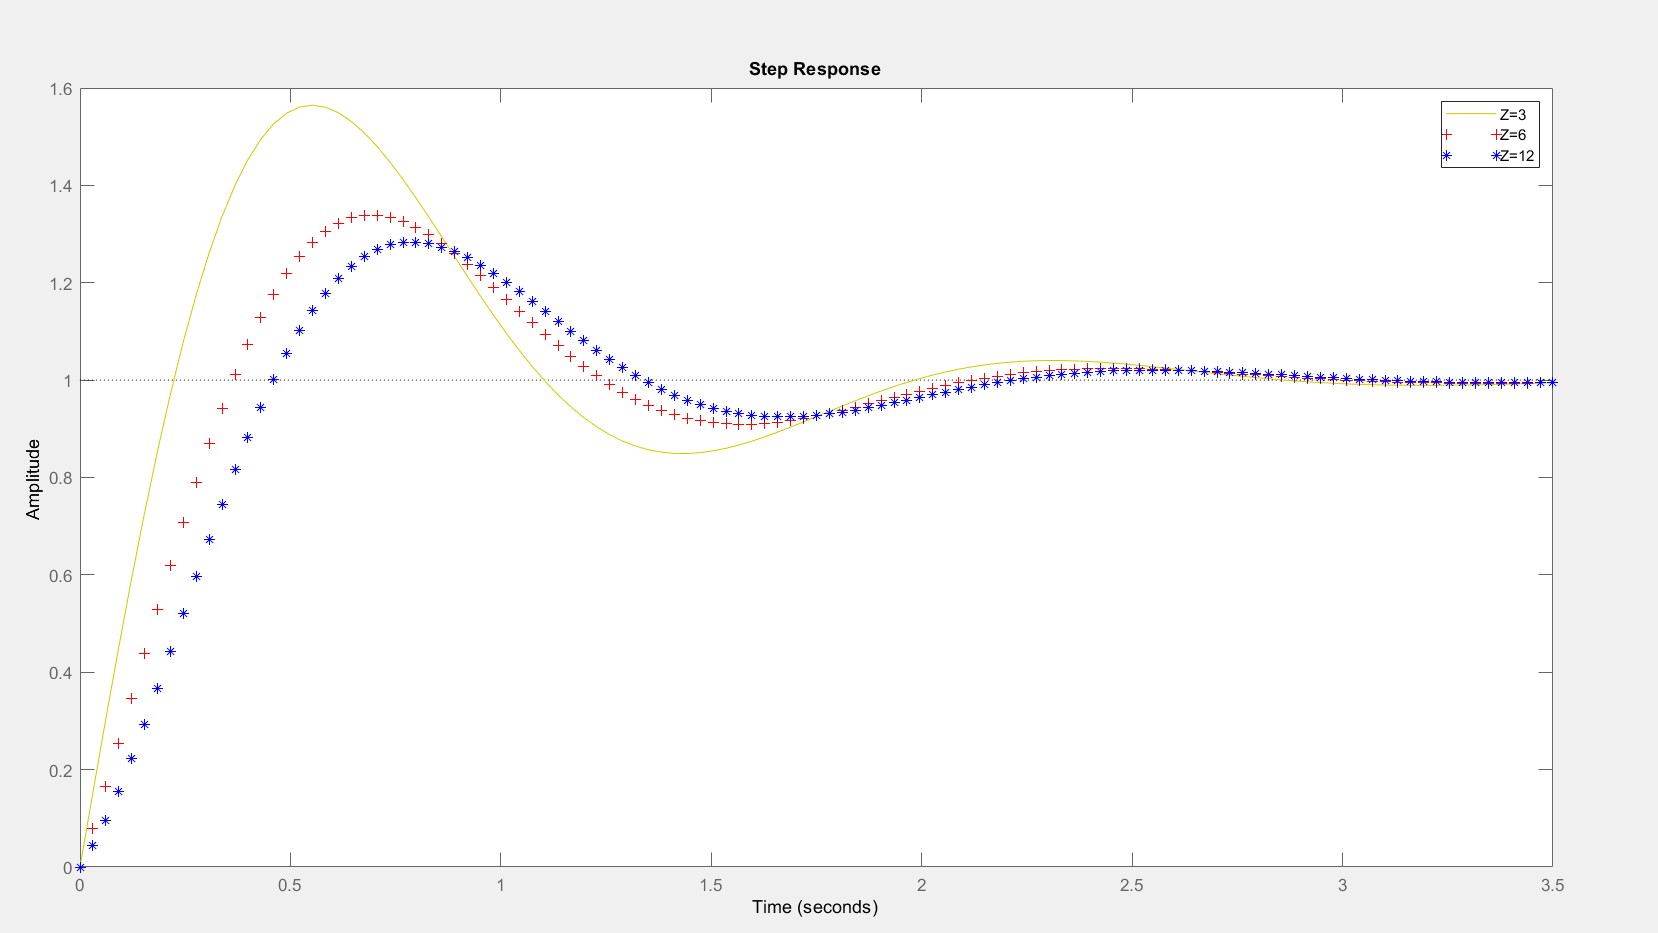
\includegraphics[scale=0.5]{../Lab6/HW0_result.png} \\



\section{Conclusion}
Today we learn the function plotting of transfer function and more ways to calculate the feedback loops for a certain transfer functions.Now we have successfully plot out almost everything we taught during Signal and System courses and those taught in Engineering math.As always these operations performed on the transfer function and graph plotting is essential for future usages, otherwise more advanced topics cannot be grasped easily without these prerequisite~

\begin{center} 
This concludes the fourth Week of Auto Control LAB\\
\end{center}

\end{document} 
